Reinforcement learning (RL) is an approach in artificial intelligence for goal-directed learning from interaction and experience. This makes it different from the other approaches in machine learning in which the learner, the decision maker, or the so-called agent, is told what to do. In reinforcement learning the agent tries out different actions in order to understand which of them generates the most reward. The reward is a special term in reinforcement learning and describes the goal in a Markov decision process (MDP) model. Roughly speaking, the MDP model would very well characterize the agent’s view of the world, the actions that it can take in the world and its goal.

Machine learning distinguishes supervised from unsupervised learning paradigms by having the supervisor indicating the correct behavior in certain generalized situations for the supervised learning and finding hidden structure in unlabeled data for the unsupervised learning. Reinforcement learning is sometimes classified as an unsupervised learning problem because it doesn’t make use of labeled data, however, it doesn’t look for structure, but tries to maximize the reward. Therefore, reinforcement learning is considered another paradigm in machine learning, according to the opinion and points of the authors R. S. Sutton and A. G. Barto of the book “An Introduction to Reinforcement Learning” \cite{Sutton}. The diagram in \Cref{fig:RLandML} illustrates the relationship between machine learning and reinforcement learning.
\begin{figure}[H]
	\centering
	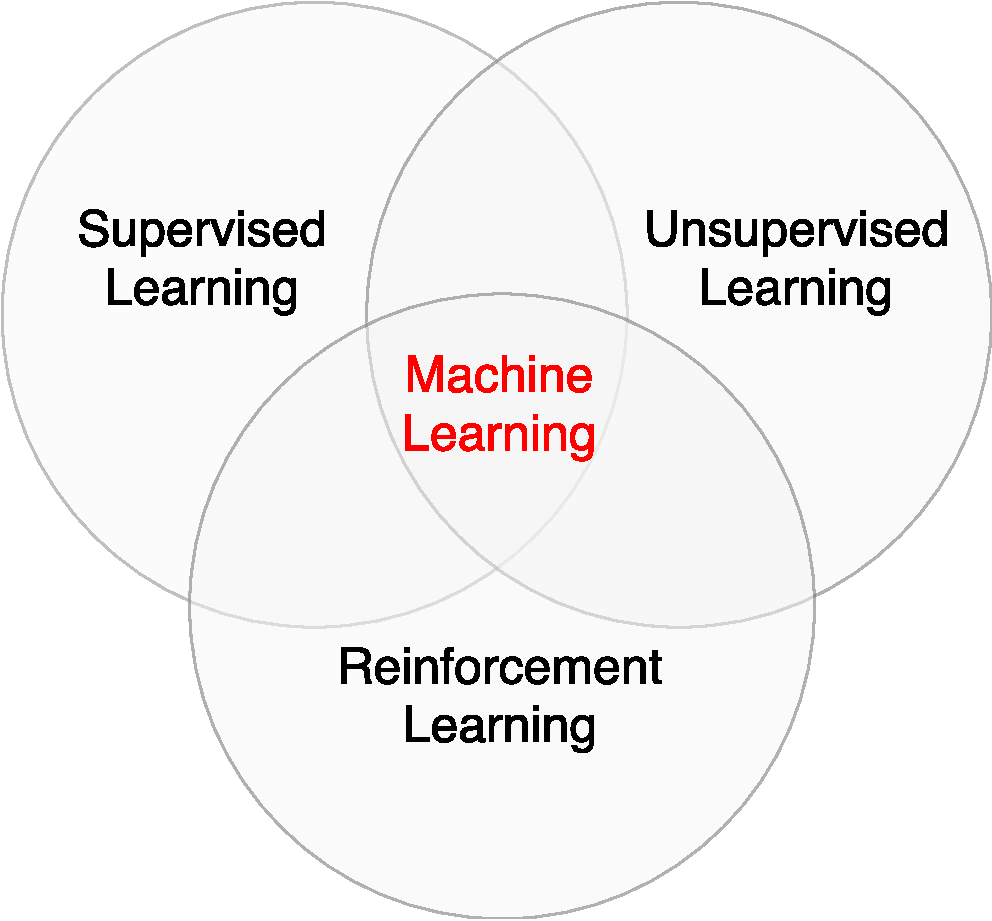
\includegraphics[width=0.7\textwidth]{Figures/RLandML}
	\caption{Reinforcement Learning and Machine Learning}
	\label{fig:RLandML}
\end{figure}
Reinforcement learning considers the problem of planning in real-time decision making and the models for prediction related to planning. The interactive goal-directed agent is able to operate in an uncertain setup, make decisions despite uncertainty and predict future events. The agent is not necessarily a robot; it can be any component in a larger system in which it interacts directly with the system and indirectly with the system’s environment. The environment is everything that the agent interacts with, it is the outer world.

There is a special concern in reinforcement learning which is not present in the other machine learning approaches. It is the issue of balancing exploitation of the knowledge that the agent has and exploration of new information in order to improve the current knowledge base.

A variety of different scientific fields intersects with reinforcement learning, especially mathematics, namely, statistics and optimization, which have an important background contribution to the reinforcement learning methods. “For example, the ability of some reinforcement learning methods to learn with parameterized approximators addresses the classical “curse of dimensionality” in operations research and control theory” \cite{Sutton}. The relationship between reinforcement learning and optimization can be exemplified by the idea of maximization of the reward signal. Actually, in reinforcement learning the agent intends to maximize the reward, but not necessarily achieves the maximum. Reinforcement learning is also part of the engineering and computer science subjects. The related algorithms have a close resemblance to the biological brain systems of animals and humans due to the reward factor involved, therefore it also binds with the psychology and neuroscience fields. The diagram in \Cref{fig:RLandOther} illustrates how reinforcement learning relates to other scientific disciplines.
\begin{figure}[H]
	\centering
	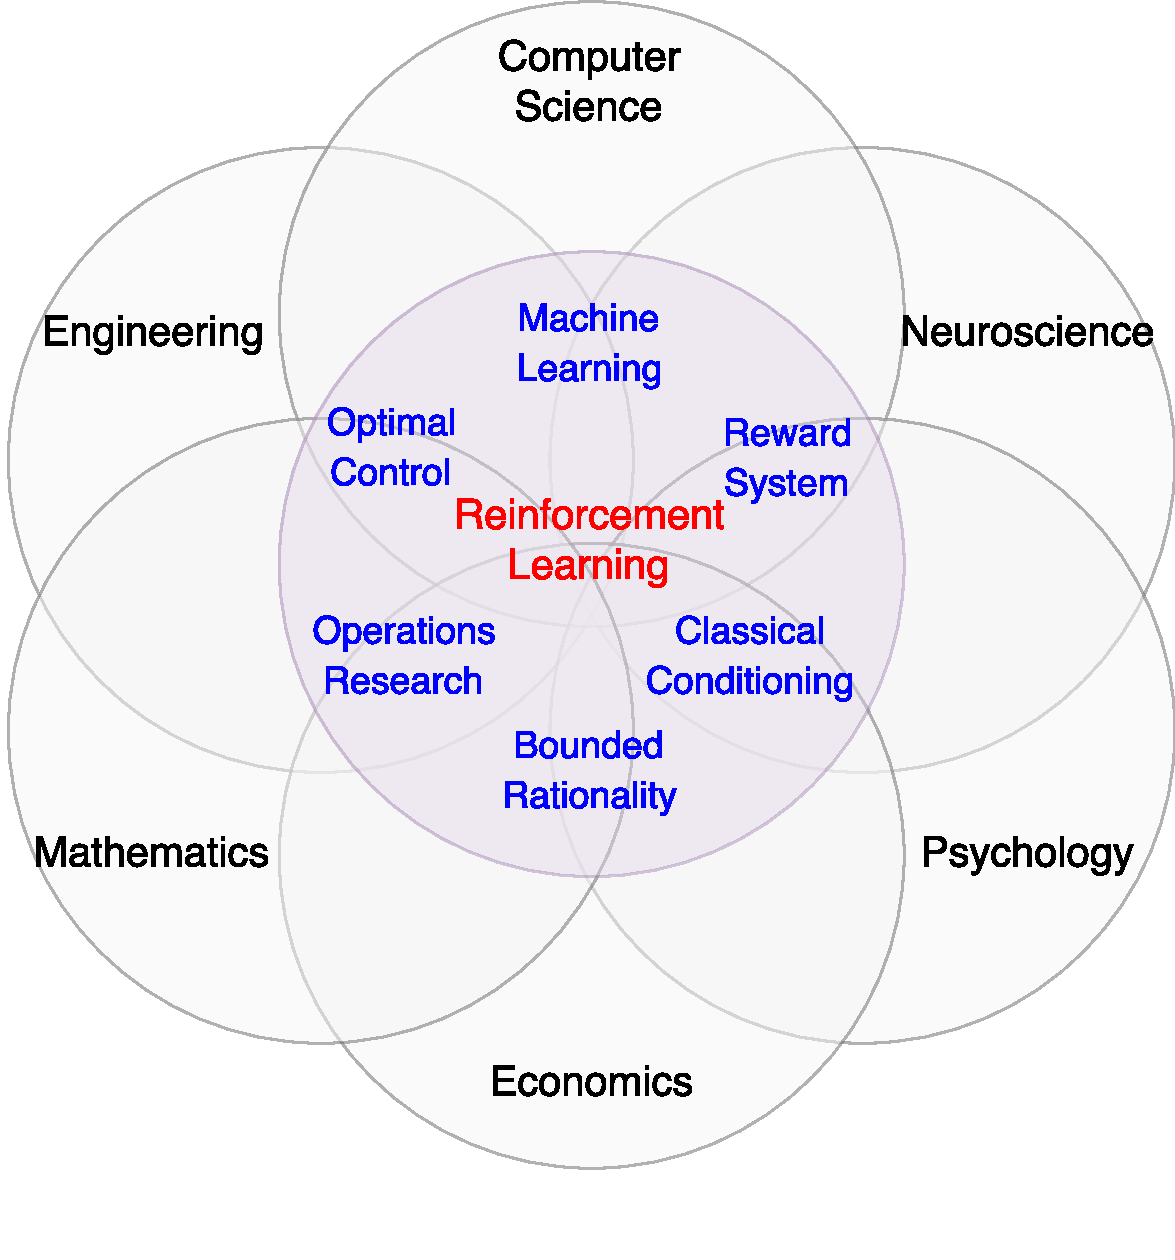
\includegraphics[width=0.7\textwidth]{Figures/RLandOther}
	\caption{Reinforcement Learning and other disciplines}
	\label{fig:RLandOther}
\end{figure}
\section{Elements of an RL problem}\label{ElementsRLproblem}
A reinforcement learning problem contains at least one of the elements: reward signal, value function, policy, environment model.

The reward signal represents a feedback from the environment as a response to the agent’s behavior in that environment, therefore the agent cannot change the feedback that it receives, but it can behave accordingly so as to maximize the gained reward signals during its lifetime. The “reward signal defines the goal in a reinforcement learning problem” \cite{Sutton}. It serves as a problem definition and as a basis for modifying the policy.

The policy maps states to actions so that when the agent is in a specific state, it chooses an action based on the defined policy. A policy is enough to describe the behavior of the agent and therefore, it is the core of reinforcement learning.

The value function provides values for judging the quality of a state based on the estimated maximum reward it can yield in the long run, in contrast with the reward which expresses only the immediate advantage of being in a specific state.

The model is a representation of the environment’s behavior. In a model-free reinforcement learning (trial-and-error) problem the agent cannot plan its future because it doesn’t have a model basis, whereas in model-based problems the agent can plan its future actions based on the environment’s modeled behavior and expected rewards in certain states.

\section{Markov Decision Processes in RL}\label{MDPs}
The general reinforcement learning problem formulation has the format of a finite MDP. The interaction between the agent and environment happens at each time step of a sequence of discrete time steps, $t=0,1,2,3,...$, where at each time step $t$ the agent receives a representation of the world - a state, $S_{t}\in S$, from a set of possible states $S$, selects an action $A_{t}$ from a set of possible actions $A(S_{t})$ for the state $S_{t}$ by implementing a policy $\pi_{t}$, where $\pi_{t}(a|s)$ is the probability that $A_{t}=a$ if $S_{t}=s$, and in the next time step $t+1$ the agent receives a reward signal $R_{t+1}\in R$ from the environment ending up in a new state $S_{t+1}$ \cite{Sutton}. The diagram in \Cref{fig:AgentEnv} illustrates the interaction between the agent and the environment.
\begin{figure}[H]
	\centering
	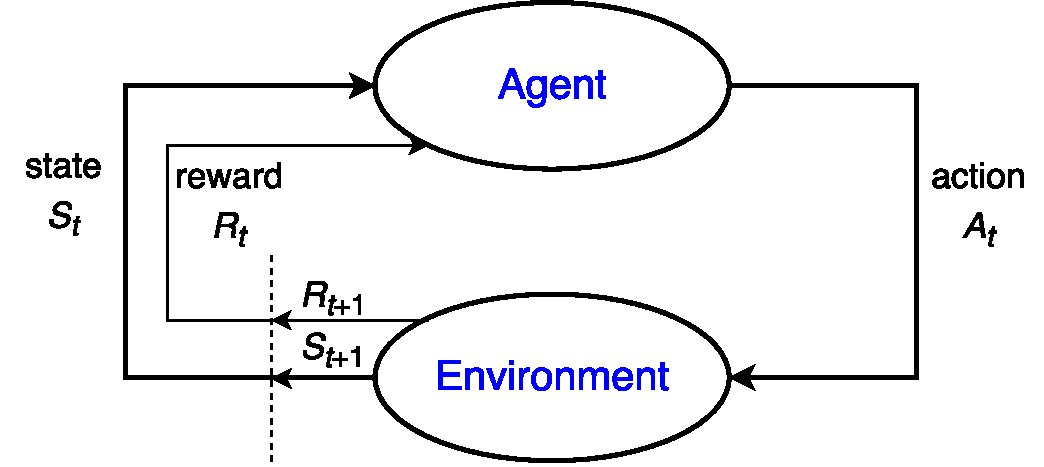
\includegraphics[width=0.7\textwidth]{Figures/Agent-EnvironmentInteraction}
	\caption{Agent - environment interaction}
	\label{fig:AgentEnv}
\end{figure}
Reinforcement learning methods provide ways to adjust the policy based on the accumulated experience with the goal of maximizing the total cumulative reward in mind. An example for representing the goal in a reinforcement learning problem like that of making a robot learn to walk would be by giving a reward on each time step proportional to the robot's forward motion. “The reward signal is your way of communicating to the robot \textit{what} you want it to achieve, not \textit{how} you want it achieved” \cite{Sutton}.

A formal definition of the cumulative reward received in the long run is expressed by the expected return $G_{t}$, which is a function of rewards sequence $R_{t+1},R_{t+2},...,R_{T}$ received after the time step $t$, where $T$ is the last time step. In order to express the return more conveniently the concept of \textit{discounting} is introduced, which determines the current value of the future rewards. The formula generalized for both episodic and continuing tasks is the following: 
\begin{equation}
G_{t}=R_{t+1}+\gamma R_{t+2}+\gamma ^2R_{t+3}+...=\sum_{k=0}^{T-t-1}\gamma ^kR_{t+k+1}, 
\end{equation}
where $\gamma$ is the discount rate, $0\leq \gamma\leq1$. In the case of episodic tasks where there is a terminal state after some time steps, $\gamma=1$. For the cases in which the process is continuous and the final step is infinite, $T=\infty$. 

With the discounting factor, the reward received after $k$ time steps has the value "$\gamma ^{k-1}$ times what it would be worth if it were received immediately" \cite{Sutton}. In the extreme point where $\gamma=0$, it is said that the agent is myopic, because it only maximizes over the immediate rewards and not the future rewards, whereas if $\gamma$ is closer to $1$ the agent is farsighted and sees far into the future considering the future rewards when picking actions.

The \textit{state} that has the Markov property represents all the useful information in order to make a sufficient statistic for the future. With Markov states we have the best possible basis for choosing action \cite{Sutton}. The environment's feedback at time step $t+1$ after a particular action was taken at time step $t$ depends on the events happened before. If the state has the Markov property instead, then the feedback of the environment depends only on that state, because that state represents all the previous events. In this case the one step environment dynamics of a finite MDP can be expressed by the following formula:
\begin{equation}\label{psrsa}
p(s',r|s,a)=Pr\left \{ S_{t+1}=s',R_{t+1}=r|S_{t}=s,A_{t}=a \right \}
\end{equation}
Based on the formula presented in (\ref{psrsa}) we can also compute the expected rewards for state-action pairs \cite{Sutton},
\begin{equation}
r(s,a)=\mathop{{}\mathbb{E}}\left [ R_{t+1}|S_{t}=s,A_{t}=a \right ]=\sum_{r\in R}r\sum_{s'\in S}p(s',r|s,a)
\end{equation}
the \textit{state-transition probabilities}
\begin{equation}
p(s'|s,a)=Pr\left \{ S_{t+1}=s'|S_{t}=s,A_{t}=a \right \}=\sum_{r\in R}p(s',r|s,a)
\end{equation}
and the expected rewards for state-action-next-state triples,
\begin{equation}
r(s,a,s')=\mathop{{}\mathbb{E}}\left [ R_{t+1}|S_{t}=s,A_{t}=a,S_{t+1}=s' \right ]=
\frac{\sum_{r\in R}rp(s',r|s,a)}{p(s'|s,a)}
\end{equation}
Value functions estimate how good it is to be in a specific state given the expected return and the policy.

The \textit{state-value function} for policy $\pi$, $v_{\pi }$ expresses the expected value of a random variable given the followed policy $\pi$ at any time step $t$:
\begin{equation}
v_{\pi }(s)=\mathop{{}\mathbb{E}_{\pi}}\left [G_{t}|S_{t}=s \right ]=\mathop{{}\mathbb{E}_{\pi}}\left [ \sum_{k=0}^{\infty}\gamma ^kR_{t+k+1} |S_{t}=s\right ]
\end{equation}

The \textit{action-value function} for policy $\pi$, $q_{\pi }$ is the value of taking an action $a$ in a state $s$ while following the policy $\pi$:
\begin{equation}
q_{\pi }(a,s)=\mathop{{}\mathbb{E}_{\pi}}\left [G_{t}|S_{t}=s,A_{t}=a \right ]=\mathop{{}\mathbb{E}_{\pi}}\left [ \sum_{k=0}^{\infty}\gamma ^kR_{t+k+1} |S_{t}=s,A_{t}=a\right ]
\end{equation}

Value functions have the property of being expressed recursively. The recursive representation is actually the \textit{Bellman equation} and it's solution is the value of $v_{\pi }$. It is like a look ahead procedure, where the value of a current state is evaluated by looking ahead at the values that future states can offer. "The Bellman equation averages over all the possibilities, weighting each by its probability of occurring. It states that the value of the start state must equal the (discounted) value of the expected next state, plus the reward expected along the way" \cite{Sutton}:
\begin{equation}\label{StateValueFunction}
v_{\pi }(s)=\mathop{{}\mathbb{E}_{\pi}}\left [G_{t}|S_{t}=s \right ]=\sum_{a}\pi(a|s)\sum_{s',r}p(s',r|s,a)\left [ r+\gamma v_{\pi }(s') \right ]), \forall s\in S
\end{equation}
The Bellman equation represents the basis of different ways of computing, approximating, and learning $v_{\pi }$ \cite{Sutton}.

In finite MDPs, an \textit{optimal policy} $\pi_{*}$ is the policy for which its expected return for all the states is greater than or equal to the expected return of all the other policies. There can be many policies that are optimal due to their \textit{state-value function}, which evaluates the same for all the optimal policies:\begin{equation}
v_{*}(s)=\max_{\pi}v_{\pi}(s), \forall s\in S
\end{equation}

Analogically, the \textit{optimal action-value function} is formed:
\begin{equation}
q_{*}(s,a)=\max_{\pi}q_{\pi}(s,a), \forall s\in S , a \in A(s)
\end{equation}

The \textit{Bellman optimality equation} for $v_{*}$ is the value of a state on the optimal policy basis, which is the same as the expected return of the best action for that state \cite{Sutton}:
\begin{equation}\label{BellmanOptimalityVstar}
\begin{split}
v_{*}(s)&=\max_{a \in A(s)}q_{\pi*}(s,a) \\
&=\mathop{{}\mathbb{E}}\left [ R_{t+1} + \gamma v_{*}(S_{t+1})|S_{t}=s, A_{t}=a  \right ] \\
&=\max_{a \in A(s)}\sum_{s',r}p(s',r|s,a)\left [ r+\gamma v_{*}(s') \right ]
\end{split}
\end{equation}

And the \textit{Bellman optimality equation} for $q_{*}$ is the following:
\begin{equation}\label{BellmanOptimalityQstar}
\begin{split}
q_{*}(s,a)&=\mathop{{}\mathbb{E}}\left [ R_{t+1} + \gamma \max_{a'}q_{*}(S_{t+1},a')|S_{t}=s, A_{t}=a  \right ] \\
&=\sum_{s',r}p(s',r|s,a)\left [ r+\gamma\max_{a'}q_{*}(s',a') \right ]
\end{split}
\end{equation}

The Bellman optimality equation generates a system of $N$ nonlinear equations, where $N$ is the number of states. It can be simply solved by applying some nonlinear methods when the system dynamics ($p(s',r|s,a)$) are known. The solution to the Bellman optimality equation helps in defining the optimal policy; e.g. one can, at any state, choose the action that corresponds to the maximum return, which is also valid in the long term, because the values take into account the reward consequences of all possible future behavior options \cite{Sutton}. In the case of the action-value pairs, if the system's dynamics are unknown, then the actions would still be optimal because the agent would choose the actions that would maximize $q_{*}$.